\subsection{Introducing Deepfield}
% Source page: Deepfield.md Page 1; exactly one frame.
\setsource{}
\begin{frame}[c,label=md-1]
\sectiondivider{Deepfield}{An AI-driven Nuclear Astrophysics Laboratory}
\end{frame}

% Source page: Deepfield.md Page 3; exactly one frame.
\setsource{\href{https://science.nasa.gov/mission/hubble/science/universe-uncovered/hubble-deep-fields/}{NASA Science: Hubble\textquotesingle s Deep Fields}}
\begin{frame}[c,label=md-3]{Name: Why Deepfield?}
\footnotesize
\begin{columns}[T,onlytextwidth]
\begin{column}{0.62\textwidth}
    \raggedright
    \setlength{\parindent}{0pt}
    \begin{itemize}
        \setlength{\itemsep}{0.4em}
        \item \textbf{Deep $\rightarrow$ nuclear;}\quad
        \textbf{Field $\rightarrow$ astrophysics.}
        \item \textbf{Deep / Field $\rightarrow$ depth / ground:}\\
        Jinping's deep underground laboratory.
        \item \textbf{Hubble Deep Field (HDF).}
        \par\medskip
        \textbf{The Hubble Deep Field experiment}\par
        In 1995, Robert Williams proposed observing an apparently empty
        patch of sky:
        \par\smallskip

        \textbf{What would we discover if we observed it for long enough?}
        \par\smallskip

        Ten days of observations in Ursa Major revealed
        \textbf{about 3,000 galaxies}.
        \par\medskip

        \textbf{Significance:} From studying known targets to exploring unknown
        regions---how do search strategies and resource allocation shape discovery?
    \end{itemize}
\end{column}
\begin{column}{0.34\textwidth}
    \begin{figure}
    \centering
    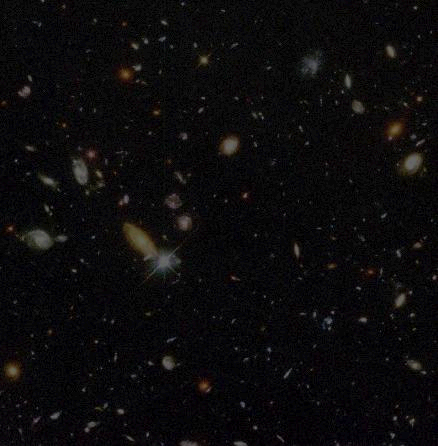
\includegraphics[width=\linewidth]{hubble_deep_field.png}
    \caption{Central portion of the Hubble Deep Field, observed in 1995.}
    \end{figure}
    {\scriptsize\itshape NASA, Robert Williams, and the Hubble Deep Field
    Team (STScI).\par}
\end{column}
\end{columns}
\end{frame}

% Source page: Deepfield.md Page 39; exactly one frame.
\setsource{}
\begin{frame}[c,label=md-39]{Deepfield Research Proposal}
\small
\begin{block}{An AI-Driven, Human-in-the-Loop Laboratory}
\textbf{Setting:} JUNA / Jinping deep underground nuclear astrophysics experiments.
\end{block}
\medskip
\textbf{Research Vision}
\begin{enumerate}
    \renewcommand{\theenumi}{\arabic{enumi}}
    \setbeamertemplate{enumerate item}{\insertenumlabel}
    \setlength{\itemsep}{0.5em}
    \item \textbf{Autonomous research:} Investigate literature, generate
    hypotheses, reuse and develop code, and design and analyze experiments.
    \item \textbf{Human guidance:} Scientists revise goals, contribute expertise,
    resolve disagreements, and judge key decisions.
    \item \textbf{Recursive improvement:} Use experimental feedback and
    reflection to improve knowledge, code, strategies, and model capabilities.
    \item \textbf{Scientific loop:} Connect real cross-section measurements
    with Code-proposed observations, archival analyses, or targeted simulations.
    \item \textbf{Long-term aim:} Accumulate research experience, proactively
    discover scientific questions, and improve human--AI discovery capabilities.
\end{enumerate}
\end{frame}

% Source page: Deepfield.md Page 41; exactly one frame.
\setsource{}
\begin{frame}[t,label=md-41]{Acceptance Criteria}
\small
\slideheading{For one scientist-confirmed reaction question}
\smallskip
\begin{enumerate}
\setlength{\itemsep}{0.55em}
    \item Identify evidence-grounded energy regions and competing hypotheses.
    \item Complete a physical cross-section measurement and reproducible analysis.
    \item Have Code proactively propose a discriminating observation,
    independent archival analysis, or targeted simulation.
    \item Complete the follow-up with the responsible teams and
    independently verify its results.
    \item Compare astrophysical conclusions before and after measurement.
\end{enumerate}

\slidenote{Replay supports development; prospective acceptance needs a
physical measurement. Unexecuted observing applications remain pending.
Report observations and simulations by their actual evidence type.}
\end{frame}

